\chapter{Results and Evaluation}

\section{Rendered Output}

Figure~\ref{fig:views} shows frames produced by the program's own rendering code (lines 1--316 of \texttt{main.cpp}, unmodified, compiled into a small test program that writes the $640\times480$ pixel buffer to an image). They show the 3D view only; the window title and hot/cold bar are drawn by SDL in \texttt{main} and are not included.

\begin{figure}[H]
\centering
\begin{minipage}{0.32\textwidth}\centering
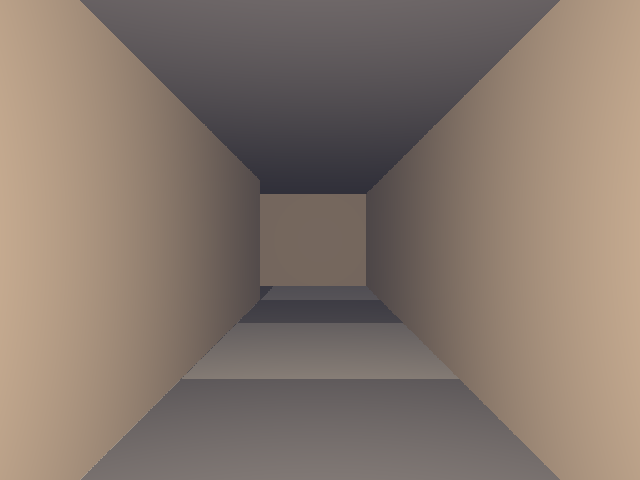
\includegraphics[width=\linewidth]{images/view_spawn.png}\\[2pt]{\small (a)}
\end{minipage}\hfill
\begin{minipage}{0.32\textwidth}\centering
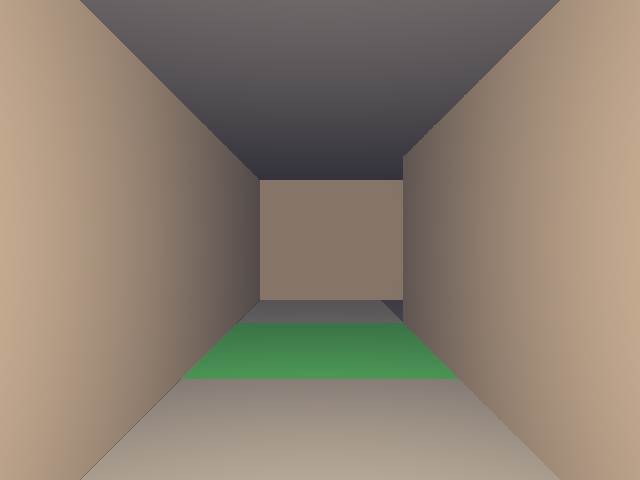
\includegraphics[width=\linewidth]{images/view_exit.png}\\[2pt]{\small (b)}
\end{minipage}\hfill
\begin{minipage}{0.32\textwidth}\centering
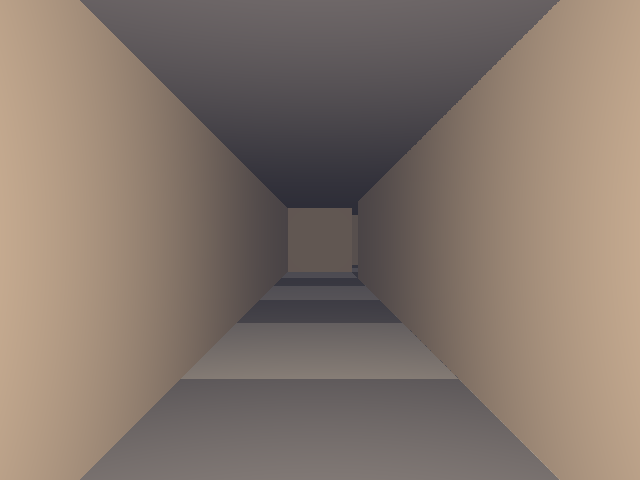
\includegraphics[width=\linewidth]{images/view_checker.png}\\[2pt]{\small (c)}
\end{minipage}
\caption{Rendered frames. (a) Spawn position $(1.5,1.5)$ facing $+x$. (b) From $(4.5,9.5)$ facing $+x$: the green exit tile ahead. (c) From $(9.5,13.5)$ facing $-x$: alternating floor tiles.}
\label{fig:views}
\end{figure}

The images show perspective convergence of the corridors and correct occlusion (the grid walk returns the first wall entered); torch lighting that brightens near surfaces and fades with distance; a green tile only on the exit cell with grey neighbours; and a checkerboard floor.

\section{Collision and Performance}

Calling \texttt{collides} on the unmodified code gave: free at the spawn $(1.5,1.5)$; blocked inside the border wall $(0.5,0.5)$; blocked at $(1.5,1.2)$, which is $0.2$ from the wall and less than the radius $0.28$; and free at $(1.5,1.3)$, $0.3$ from the wall. All four match the expected result.

Each frame casts $640\times480=307{,}200$ rays. Calling \texttt{render} 30 times on one thread with \texttt{-O3} took about 11--12~ms per frame (roughly 85 frames/s) on the machine used to prepare this report; the value depends on the processor. In the game, a frame is padded to at least about 15~ms and presentation is vsynced when available, so the displayed rate is limited to about 60--66 frames/s.
